\section{Presentation Logic Layer}

%What pages will be present in your project? briefly indicate how your web site will be organized
The presentation logic layer of our web application consists of several pages that allow users to interact with the system. These pages are developed using JSP, servlets and REST technologies.
We will describe the main pages.

\subsection{Homepage}

The homepage is the main entry point for the web application. It provides users with several options to interact with the system:

\begin{itemize}
\item \textbf{Login}: Users can log in to the system by clicking on the “Login” button, which will direct them to the home page.
\item \textbf{Create Administrator}: Users can create a new administrator account by clicking on the "Create Administrator" button. This will direct them to a form where they can enter the administrator's details, including an optional profile picture.
\end{itemize}

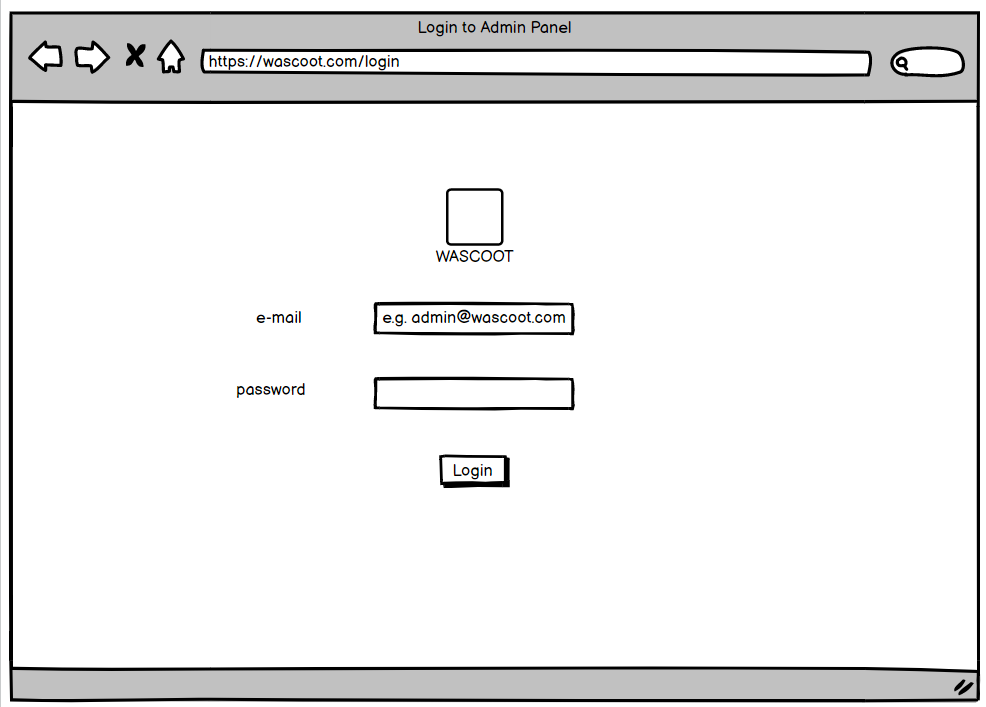
\includegraphics[scale = 0.7]{sections/DLL/Login.png}

\subsection{Dashboard}

The dashboard is the main page of the web application. It provides users with an overview of their business data and allows them to visualize this data in various ways. The dashboard is developed using JSP and REST technologies.

On the dashboard, users can view the following information:

\begin{itemize}
\item \textbf{Scooter rack Locations}: Users can view the locations of their scooter racks on a map, along with information about each rack, such as its capacity and availability.
\item \textbf{Revenue}: Users can view their business revenue over a specified period.
\item \textbf{Top Locations}: Users can view a list of their top-performing locations based on their utilization.
\item \textbf{Customer Information}: Users can view information about their customers, including age, rental history, and gender.
\end{itemize}

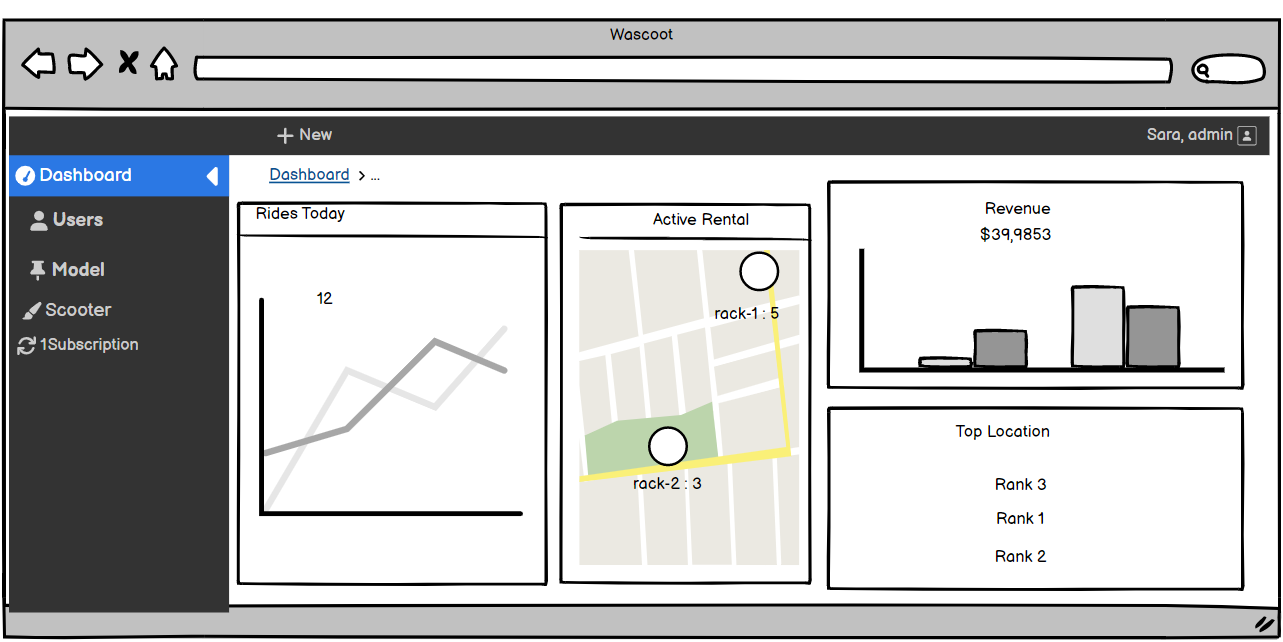
\includegraphics[scale = 0.6]{sections/DLL/Dashboard.png}

\subsection{Manage Pages}

In addition to the homepage and dashboard, our web application includes several manage pages that allow users to modify and create data. These pages are developed using JSP and REST technologies.

\subsubsection{Model Page}

The model page allows users to view information about scooter models and to modify or create new models through a form. The following pages are available:

\begin{itemize}
\item \textbf{Show Models}: Users can view a list of all scooter models in the system, along with information such as the model name, brand, and specifications.
\item \textbf{Modify Model}: Users can modify an existing scooter model by selecting it from the list and editing its information in a form.
\item \textbf{Create Model}: Users can create a new scooter model by filling out a form with the model's details.
\end{itemize}

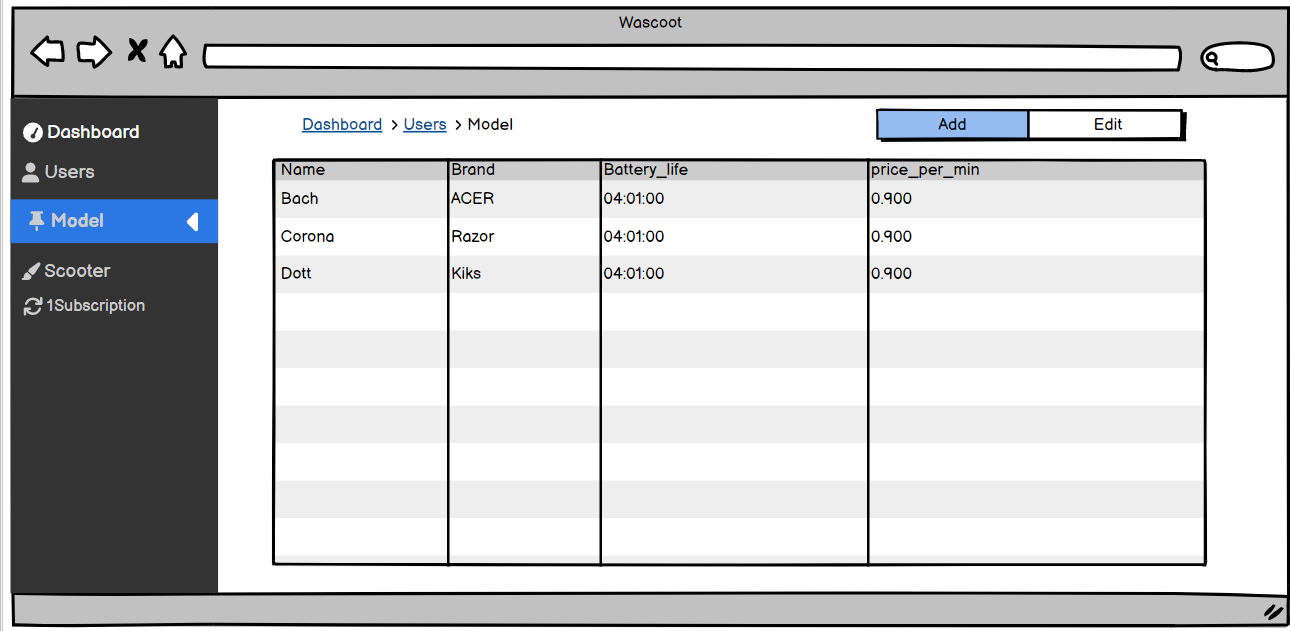
\includegraphics[scale = 0.7]{sections/DLL/Model.png}

\subsubsection{Scooter Page}

The scooter page allows users to view information about scooters and to modify or create new scooters through a form. The following pages are available:

\begin{itemize}
\item \textbf{Show Scooters}: Users can view a list of all scooters in the system, along with useful information.
\item \textbf{Modify Scooter}: Users can modify an existing scooter by selecting it from the list and editing its information in a form.
\item \textbf{Create Scooter}: Users can create a new scooter by filling out a form with the scooter's details.
\end{itemize}

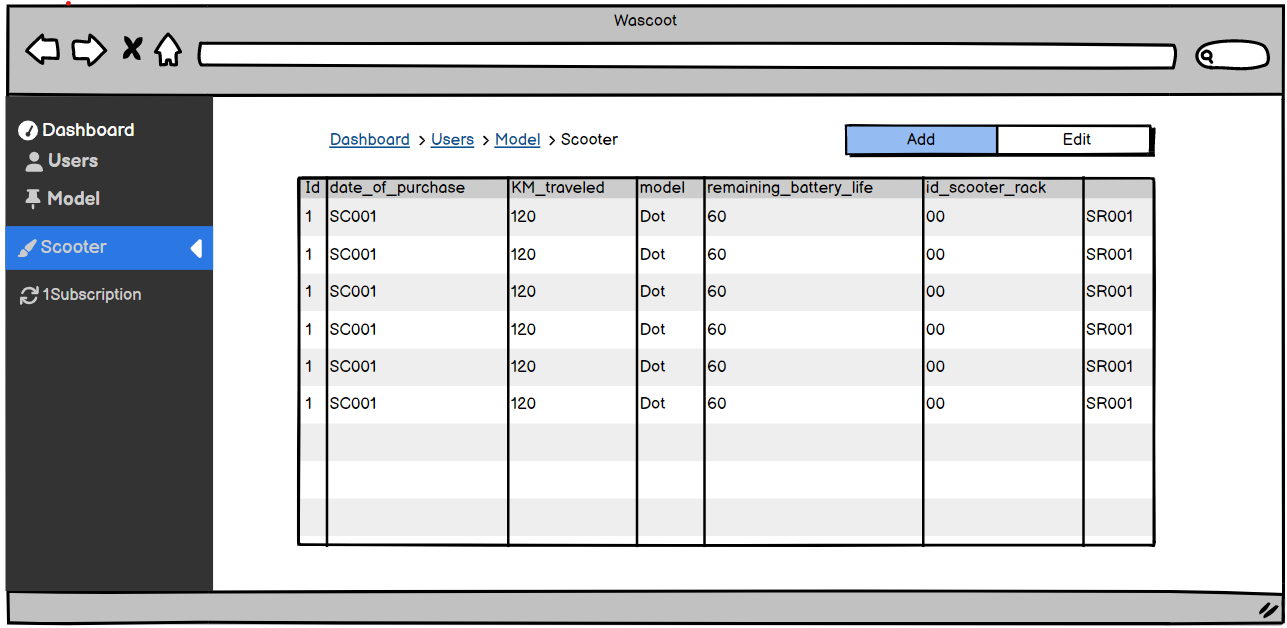
\includegraphics[scale = 0.6]{sections/DLL/Scooter.png}

\subsection{Subscription Page}

Similarly to the scooter page, we have a page to manage subscriptions.

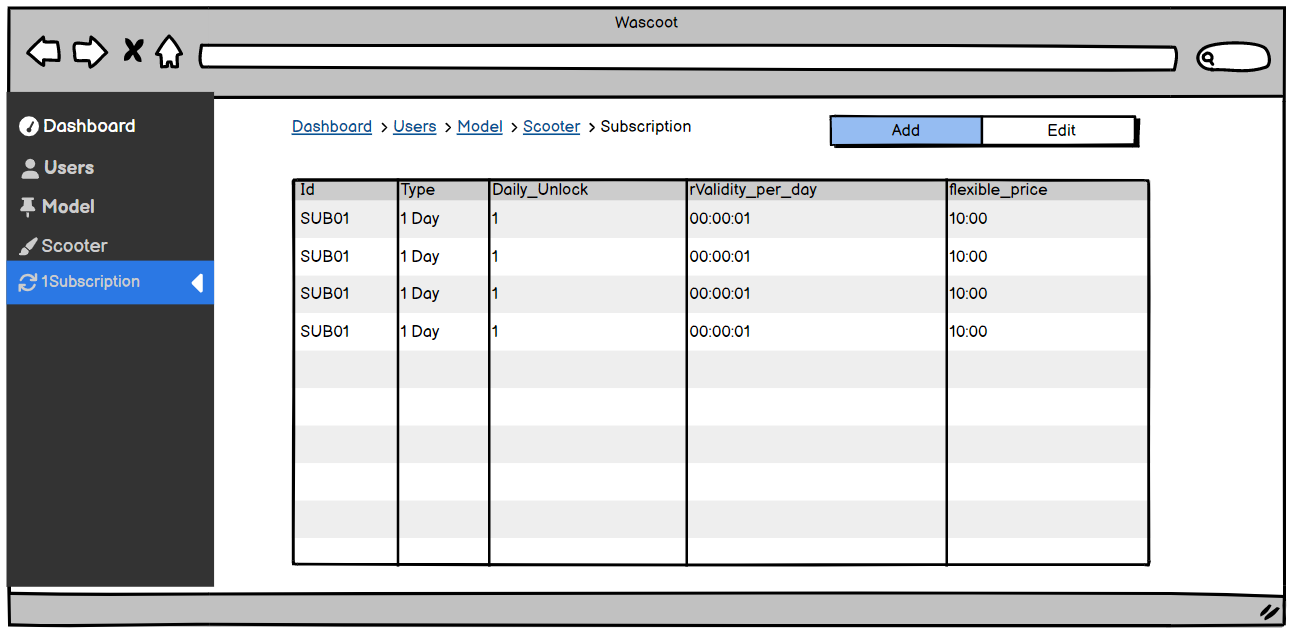
\includegraphics[scale = 0.6]{sections/DLL/subScription.png}

\subsection{Customer Page}

Similarly to scooter and subscription pages, we have a page to manage customers.

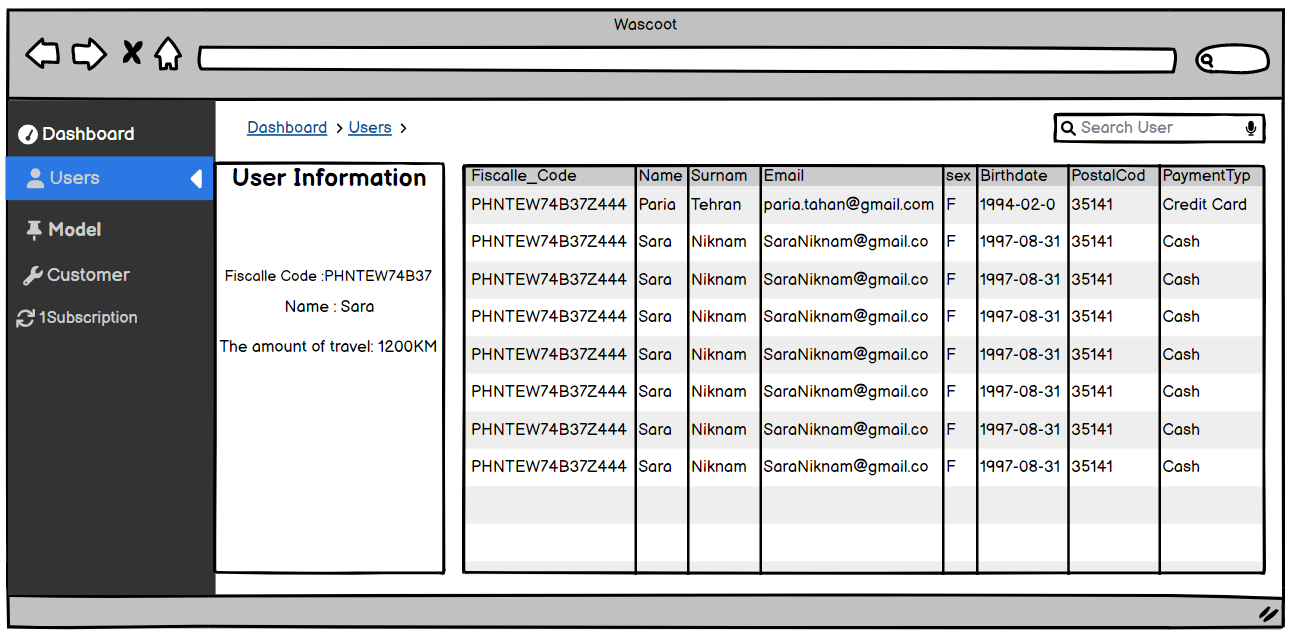
\includegraphics[scale = 0.6]{sections/DLL/Users.png}